\documentclass[letterpaper, titlepage, 10pt]{article}

\usepackage[margin=4cm]{geometry}
\usepackage[bookmarks]{hyperref} % wg. pdf indicies

\usepackage{listings} % wg. source listings

\usepackage{tikz}
\usetikzlibrary{decorations.pathreplacing}
\usetikzlibrary{decorations.markings}
\usetikzlibrary{arrows}
\usetikzlibrary{positioning} % wg. 'of' relative positioning
\usetikzlibrary{shapes.misc} % wg. 'rounded rectangle'

% style to apply some styles to each segment of a path
\tikzset{
  on each segment/.style={
    decorate,
    decoration={
      show path construction,
      moveto code={},
      lineto code={
        \path [#1]
        (\tikzinputsegmentfirst) -- (\tikzinputsegmentlast);
      },
      curveto code={
        \path [] (\tikzinputsegmentfirst)
        .. controls
        (\tikzinputsegmentsupporta) and (\tikzinputsegmentsupportb)
        ..
        (\tikzinputsegmentlast);
      },
      closepath code={
        \path [#1]
        (\tikzinputsegmentfirst) -- (\tikzinputsegmentlast);
      },
    },
  },
  % style to add an arrow in the middle of a path segment
  mid arrow/.style={
    postaction={
      decorate,
      decoration={
        markings,
        % Draw arrows manually to get them centered correctly, because this
        % isn't the default behavior for TIKZ
        mark=at position 0.5 with {
          \fill (2pt,0)--(-2pt,2.31pt)--(-2pt,-2.31pt)--cycle;
        }
      }
    }
  }
}

% path styling
\tikzset {
  syntax path/.style = {
    draw = black,
    rounded corners = 2mm
  },
  arrs/.style = {
    syntax path,
    postaction = {
      on each segment = {
        mid arrow
      }
    }
  },
  % path style adds an arrow to each segment
  arr/.style = {
    syntax path,
    postaction = {
      mid arrow
    }
  },
  % path style with no arrows
  narr/.style = {
    syntax path
  }
}

% node styling
\tikzset {
  syntax node/.style = {
    draw = black,
    inner sep = 0.2cm
  },
  % terminal symbol
  term/.style = {
    syntax node,
    rounded rectangle,
    font = \ttfamily
  },
  % non-terminal symbol
  nterm/.style = {
    syntax node,
    rectangle,
    font = \itshape
  },
  % support node
  entry/.style = {
    draw = black,
    circle,
    thick,
    minimum size = .2cm,
    inner sep = 0
  },
  exit/.style = {
    entry
  },
  node distance = 0.5cm
}

\title{Syntax Documentation}
\date{}

\begin{document}

\maketitle

\section{Declaration Blocks}

\subsection{Program}

A full program; the entrying point of a parse.

\begin{figure}[h]
  \centering

  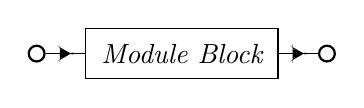
\begin{tikzpicture}
    \node[entry] (entry) {};
    \node[nterm] (mod) [right=of entry] {Module Block};
    \node[exit] (exit) [right=of mod] {};

    \draw[arr] (entry) -- (mod);
    \draw[arr] (mod) -- (exit);
  \end{tikzpicture}
\end{figure}

\subsection{Module Block}

One or more modules.

\begin{figure}[h]
  \centering
  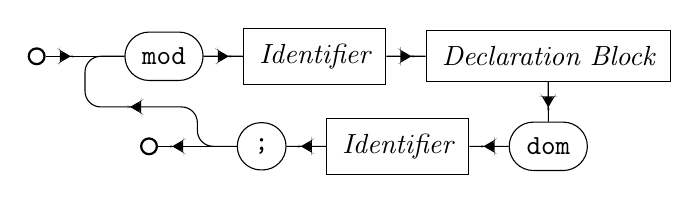
\begin{tikzpicture}
    \node[entry] (entry) {};
    \coordinate[right=of entry] (entry-mod);
    \node[term] (mod) [right=of entry-mod] {mod};
    \node[nterm] (name) [right=of mod] {Identifier};
    \node[nterm] (decl) [right=of name] {Declaration Block};
    \node[term] (dom) [below=of decl] {dom};
    \node[nterm] (exit name) [left=of dom] {Identifier};
    \node[term] (semi) [left=of exit name] {;};
    \coordinate[left=of semi] (semi-exit);
    \node[exit] (exit) [left=of semi-exit] {};

    \draw[arr] (entry) -- (entry-mod);
    \draw[narr] (entry-mod) -- (mod);

    \draw[arrs] (mod)
      -- (name)
      -- (decl)
      -- (dom)
      -- (exit name)
      -- (semi);

    \draw[narr] (semi) -- (semi-exit);
    \draw[arr] (semi-exit) -- (exit);

    \draw[arr] (semi)
      -- (semi-exit)
      -- ++(0, 0.5)
      -| (entry-mod)
      -- (mod);
  \end{tikzpicture}
\end{figure}

\subsection{Declaration Block}

A series of declarations

\begin{figure}[h]
  \centering
  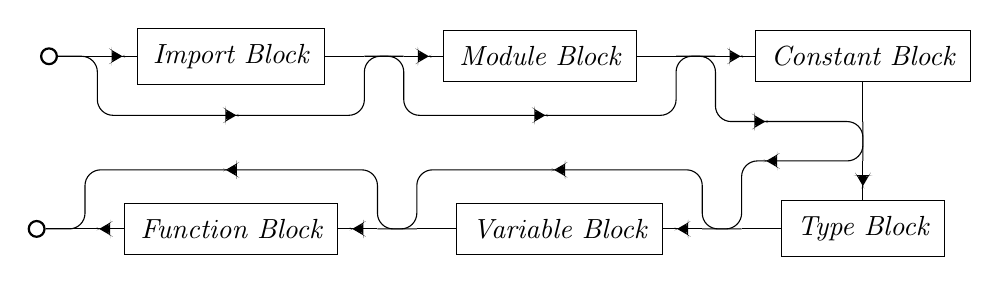
\begin{tikzpicture}
    \node[entry] (entry) {};
    \coordinate[right=of entry] (entry-imports);

    \node[nterm] (imports) [right=of entry-imports] {Import Block};
    \coordinate[right=of imports] (imports-mods 1);
    \coordinate[right=of imports-mods 1] (imports-mods 2);

    \node[nterm] (mods) [right=of imports-mods 2] {Module Block};
    \coordinate[right=of mods] (mods-consts 1);
    \coordinate[right=of mods-consts 1] (mods-consts 2);

    \node[nterm] (consts) [right=of mods-consts 2] {Constant Block};
    \coordinate[below=of consts] (consts-types 1);
    \coordinate[below=of consts-types 1] (consts-types 2);

    \node[nterm] (types) [below=of consts-types 2] {Type Block};
    \coordinate[left=of types] (types-vars 1);
    \coordinate[left=of types-vars 1] (types-vars 2);

    \node[nterm] (vars) [left=of types-vars 2] {Variable Block};
    \coordinate[left=of vars] (vars-funcs 1);
    \coordinate[left=of vars-funcs 1] (vars-funcs 2);

    \node[nterm] (funcs) [left=of vars-funcs 2] {Function Block};
    \coordinate[left=of funcs] (funcs-exit);

    \node[exit] (exit) [left=of funcs-exit] {};

    % main path
    \draw[narr] (entry) -- (entry-imports);
    \draw[arr] (entry-imports) -- (imports);
    
    \draw[narr] (imports) -- (imports-mods 1);
    \draw[arr] (imports-mods 2) -- (mods);

    \draw[narr] (mods) -- (mods-consts 1);
    \draw[arr] (mods-consts 2) -- (consts);

    \draw[narr] (consts) -- (consts-types 1);
    \draw[arr] (consts-types 2) -- (types);
      
    \draw[narr] (types) -- (types-vars 1);
    \draw[arr] (types-vars 2) -- (vars);

    \draw[narr] (vars) -- (vars-funcs 1);
    \draw[arr] (vars-funcs 2) -- (funcs);

    \draw[arr] (funcs) -- (funcs-exit);
    \draw[narr] (funcs-exit) -- (exit);
    
    % side path
    \draw[arr] (entry)
      -- (entry-imports)
      -- ++(0, -0.75)
      -| (imports-mods 1)
      -- (imports-mods 2);

    \draw[arr] (imports-mods 1)
      -- (imports-mods 2)
      -- ++(0, -0.75)
      -| (mods-consts 1)
      -- (mods-consts 2);

    \draw[arr] (mods-consts 1)
      -- (mods-consts 2)
      |- (consts-types 1)
      -- (consts-types 2);

    \draw[arr] (consts-types 1)
      -- (consts-types 2)
      -| (types-vars 1)
      -- (types-vars 2);

    \draw[arr] (types-vars 1)
      -- (types-vars 2)
      -- ++(0, 0.75)
      -| (vars-funcs 1)
      -- (vars-funcs 2);

    \draw[arr] (vars-funcs 1)
      -- (vars-funcs 2)
      -- ++(0, 0.75)
      -| (funcs-exit)
      -- (exit);
  \end{tikzpicture}
\end{figure}

\newpage
\section*{Earlier version of Module Block}

\begin{figure}[h]
  \centering
  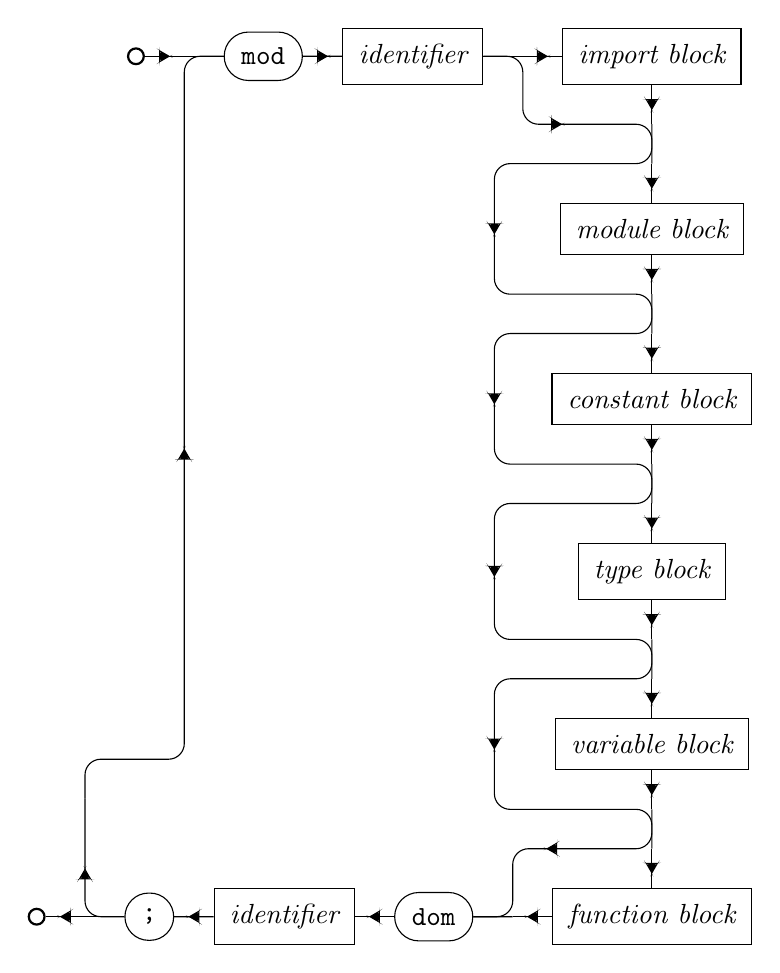
\begin{tikzpicture}
    \node[entry] (entry) {};

    \coordinate[right=of entry] (entry-mod);

    \node[term] (mod) [right=of entry-mod] {mod};
    \node[nterm] (mod name) [right=of mod] {identifier};

    \coordinate[right=of mod name] (name-imports);

    \node[nterm] (imports) [right=of name-imports] {import block};

    \coordinate[below=of imports] (imports-mods1);
    \coordinate[below=of imports-mods1] (imports-mods2);

    \node[nterm] (mods) [below=of imports-mods2] {module block};

    \coordinate[below=of mods] (mods-consts1);
    \coordinate[below=of mods-consts1] (mods-consts2);

    \node[nterm] (consts) [below=of mods-consts2] {constant block};

    \coordinate[below=of consts] (consts-types1);
    \coordinate[below=of consts-types1] (consts-types2);

    \node[nterm] (types) [below=of consts-types2] {type block};

    \coordinate[below=of types] (types-vars1);
    \coordinate[below=of types-vars1] (types-vars2);

    \node[nterm] (vars) [below=of types-vars2] {variable block};

    \coordinate[below=of vars] (vars-funcs1);
    \coordinate[below=of vars-funcs1] (vars-funcs2);

    \node[nterm] (funcs) [below=of vars-funcs2] {function block};

    \coordinate[left=of funcs] (funcs-dom);

    \node[term] (dom) [left=of funcs-dom] {dom};
    \node[nterm] (mod name exit) [left=of dom] {identifier};

    \node[term] (semi) [left=of mod name exit] {;};

    \coordinate[left=of semi] (semi-exit);

    \node[entry] (exit) [left=of semi-exit] {};

    % main line
    \draw[arr] (entry) -- (entry-mod);
    \draw[narr] (entry-mod) -- (mod);
    \draw[arr] (mod) -- (mod name);

    \draw[narr] (mod name) -- (name-imports);
    \draw[arr] (name-imports) -- (imports);

    \draw[arr] (imports) -- (imports-mods1);
    \draw[arr] (imports-mods2) -- (mods);

    \draw[arr] (mods) -- (mods-consts1);
    \draw[arr] (mods-consts2) -- (consts);

    \draw[arr] (consts) -- (consts-types1);
    \draw[arr] (consts-types2) -- (types);

    \draw[arr] (types) -- (types-vars1);
    \draw[arr] (types-vars2) -- (vars);

    \draw[arr] (vars) -- (vars-funcs1);
    \draw[arr] (vars-funcs2) -- (funcs);

    \draw[arr] (funcs) -- (funcs-dom);
    \draw[narr] (funcs-dom) -- (dom);

    \draw[arr] (dom) -- (mod name exit);

    \draw[arr] (mod name exit) -- (semi);

    \draw[narr] (semi) -- (semi-exit);

    \draw[arr] (semi-exit) -- (exit);

    % loop back to entry
    \draw[arr] (semi)
    -- (semi-exit)
    -- ++(0, 1.5);

    \draw[arr] (semi-exit) + (0, 1.5)
    -- ++(0, 2)
    -| (entry-mod)
    -- (mod);

    % side rail
    \draw[arr] (mod name)
      -- (name-imports)
      |- (imports-mods1)
      -- (imports-mods2);

    \draw[arr] (imports-mods1)
      -- (imports-mods2)
      -- ++(-2,0)
      |- (mods-consts1)
      -- (mods-consts2);

    \draw[arr] (mods-consts1)
      -- (mods-consts2)
      -- ++(-2,0)
      |- (consts-types1)
      -- (consts-types2);

    \draw[arr] (consts-types1)
      -- (consts-types2)
      -- ++(-2,0)
      |- (types-vars1)

      -- (types-vars2);

    \draw[arr] (types-vars1)
      -- (types-vars2)
      -- ++(-2,0)
      |- (vars-funcs1)
      -- (vars-funcs2);

    \draw[arr] (vars-funcs1)
      -- (vars-funcs2)
      -| (funcs-dom)
      -- (dom);
  \end{tikzpicture}
\end{figure}

\end{document}

